\section{Durchführung}
\label{sec:Durchführung}

\begin{figure}
    \centering
    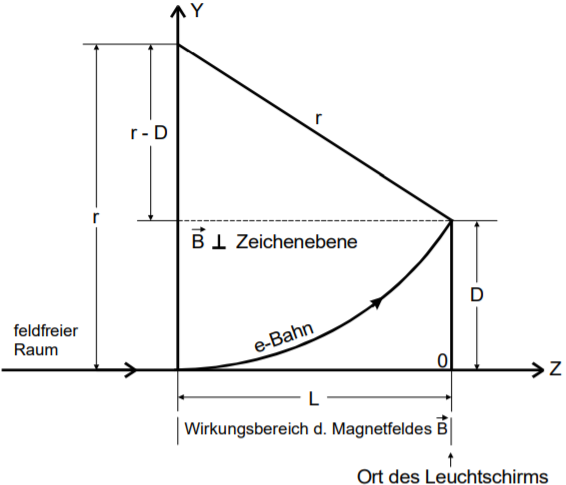
\includegraphics[width=\textwidth]{data/skizze_aufbau.png}
    \caption{skizze der Elektronenbahn im Versuchsaufbau}
    \label{fig:skizze}
\end{figure}

In der Abbildung \ref{fig:skizze} ist die schematische Funktionsweise des Versuchs dargestellt. Das homogene Magnetfeld $\vec{B}$
wird mit einer Helmholtzspule erzeugt, welche die Maße
\begin{align*}
    &\text{Anzahl der Windungen} \: N = 20 \\
    &\text{Radius der Spule} \: R_s = \SI{28.2}{\centi\m} 
\end{align*}
besitzt.
Die Helmholtzspule befindet sich auf einer um die $Y$-Achse drehbaren Vorrichtung. Damit kann diese 
so ausgerichtet werden, dass das von ihr erzeugte Magnetfeld in Richtung der Vertikalkomponente des Erdmangnetfeldes wirkt. 
Um diese Ausrichtung zu garantieren, wird ein Kompass verwendet. Auf der Drehbaren Vorrichtung befindet sich außerdem die 
Kathodenstrahlröhre, von der aus die Elektronen emittiert werden. Deren Ausrichtung ist genau senkrecht zu dem von der 
Helmholtzspule erzeugten Magnetfeld und damit in Richtung der Horizontalkomponente des Erdmangnetfeldes. Die Elektronen 
treffen am Ende des Wirkungsbereiches des Magnetfelds auf einen Schirm, auf dem am Auftreffpunkt ein Leuchtfleck erzeugt wird.\\
Infolge dieser Vorbeitungen wird eine konstante Beschleunigungsspannung $U_B$ von $\SI{250}{\volt} $ angelegt zuerst ohne ein 
Magnetfeld die Position des Leuchtflecks registriert. Daraufhin wird der Spulenstrom $I_S$, der das Magnetfeld der 
Helmholtzspule erzeugt, in $\SI{5}{\ampere} $ Schritten von $\SI{5}{\ampere} $ bis $\SI{20}{\ampere} $ erhöht und jeweils 
die zugehörige Strahlenverschiebung $D$ gemessen. Das gleiche Verfahren wird wiederholt mit $U_B$ = $\SI{380}{\volt} $. \\
Für die Bestimmung des Erdmangnetfeldes wird zuerst $U_B$ =$\SI{5}{\ampere} $ angelegt. Die Achse der Kathodenstrahlröhre
wird dann in Nord-Süd-Richtung ausgerichtet und die Position des Leuchtflecks wird notiert. Daraufhin wird die Achse in 
Ost-West-Richtung ausgerichtet, wodurch das Erdmangnetfeld eine Kraft auf die Elektronen auswirkt.
Der Spulenstrom wird nun so eingestellt, dass der Leuchtfleck sich wieder an der ursprünglichen Position befindet. In dieser 
Position kompensiert die Horizontalkomponente der Helmholtzspule genau die des Erdmangnetfeldes. 
Desweiteren muss der Inklinationswinkel $\phi$ bestimmt werden, der den Winkel zwischen der Horizontalebene und der Richtung
des Erdmangnetfeldes angibt. Der Aufbau muss dafür wieder in Nord-Süd-Richtung ausgerichtet werden. Dann wird der Kompass
um $\SI{90}{\degree} $ um seine horizontale Achse gedreht, wodurch die Magnetnadel in die exakte Richtung des Erdmangnetfeldes
zeigt. Der Winkel $\phi$ der Nadel zur Horizontalebene kann auf dem Kompass abgelesen werden. 


